% This file was created with tikzplotlib v0.10.1.
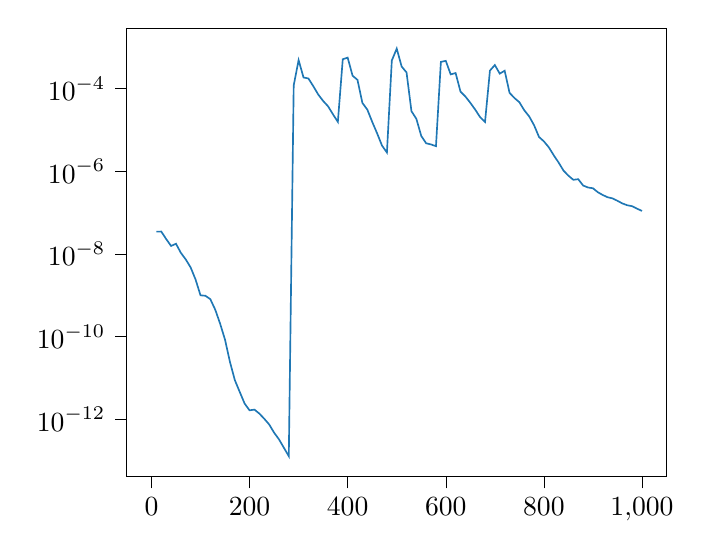
\begin{tikzpicture}

\definecolor{darkgray176}{RGB}{176,176,176}
\definecolor{steelblue31119180}{RGB}{31,119,180}

\begin{axis}[
log basis y={10},
tick align=outside,
tick pos=left,
x grid style={darkgray176},
xmin=-50, xmax=1050,
xtick style={color=black},
y grid style={darkgray176},
ymin=4.10814814321268e-14, ymax=0.00287433433030315,
ymode=log,
ytick style={color=black},
ytick={1e-16,1e-14,1e-12,1e-10,1e-08,1e-06,0.0001,0.01,1},
yticklabels={
  \(\displaystyle {10^{-16}}\),
  \(\displaystyle {10^{-14}}\),
  \(\displaystyle {10^{-12}}\),
  \(\displaystyle {10^{-10}}\),
  \(\displaystyle {10^{-8}}\),
  \(\displaystyle {10^{-6}}\),
  \(\displaystyle {10^{-4}}\),
  \(\displaystyle {10^{-2}}\),
  \(\displaystyle {10^{0}}\)
}
]
\addplot [semithick, steelblue31119180]
table {%
10 3.45097741857585e-08
20 3.46534639004363e-08
30 2.29191080397748e-08
40 1.55520814628901e-08
50 1.75828035795783e-08
60 1.05963580747827e-08
70 7.33047629798598e-09
80 4.68214669665855e-09
90 2.3921871367942e-09
100 9.95087220761903e-10
110 9.70197062745966e-10
120 8.03098676081409e-10
130 4.48989788072866e-10
140 2.05049328916811e-10
150 8.41559690710315e-11
160 2.44526181209912e-11
170 8.83330100252001e-12
180 4.56871670058274e-12
190 2.39001818698254e-12
200 1.64191464419028e-12
210 1.71062289970914e-12
220 1.36862033899076e-12
230 1.0262538199235e-12
240 7.48413947748524e-13
250 4.74207334619567e-13
260 3.26213076266586e-13
270 2.03981200766248e-13
280 1.27819082432609e-13
290 0.000118962541700681
300 0.000486615628783435
310 0.000185050100123979
320 0.000174824051756448
330 0.000113621414936695
340 7.15580047149194e-05
350 5.00361876587252e-05
360 3.72231749898276e-05
370 2.381581186314e-05
380 1.56352605488705e-05
390 0.000509951642860803
400 0.000558326173702108
410 0.000204122748105147
420 0.00016196369255184
430 4.48569567165922e-05
440 3.09297441331186e-05
450 1.56455756298339e-05
460 8.25075759203668e-06
470 4.16823645145053e-06
480 2.8290964637251e-06
490 0.000476501979607596
500 0.000923820686025741
510 0.000341146640503785
520 0.000244887080280464
530 2.83251116660145e-05
540 1.84840020562863e-05
550 7.10204583155937e-06
560 4.74002829968184e-06
570 4.43247447250699e-06
580 4.03669212107854e-06
590 0.000440345726675669
600 0.000467074508166861
610 0.000219852693277963
620 0.000236651147430587
630 8.43304015608251e-05
640 6.3991460832291e-05
650 4.51261581018564e-05
660 3.08584551489431e-05
670 2.02718066367108e-05
680 1.55634114235789e-05
690 0.000271726489908218
700 0.000369779464702584
710 0.000229206685960911
720 0.000269244697337957
730 7.86028388744415e-05
740 5.88400577491338e-05
750 4.6615649064292e-05
760 2.97352812758432e-05
770 2.11514400450307e-05
780 1.2937054177305e-05
790 6.7399957058868e-06
800 5.26538673984591e-06
810 3.78385242413927e-06
820 2.43573415671268e-06
830 1.61884898120731e-06
840 1.03198609164342e-06
850 7.79547365341946e-07
860 6.19183574174983e-07
870 6.40933683465893e-07
880 4.49523412314741e-07
890 4.0316800059044e-07
900 3.86310772881423e-07
910 3.09892145598669e-07
920 2.65524843604703e-07
930 2.34169127424963e-07
940 2.20043813215326e-07
950 1.92201611436319e-07
960 1.65988744070008e-07
970 1.49963143412913e-07
980 1.42426210831297e-07
990 1.2353839931766e-07
1000 1.09549714317097e-07
};
\path [draw=black, semithick, dash pattern=on 5.55pt off 2.4pt]
(axis cs:0,0)
--(axis cs:1000,0);

\end{axis}

\end{tikzpicture}
